\chapter{Implementace}
\label{chap:development}

V~této kapitole je popsána celková implementace modelové hry, která byla vytvořena na základě stanovených požadavků a~návrhu herního systému, popsaných v~předchozích kapitolách.

Hybridní deskové hře, která je finálním produktem této práce, bylo určeno pracovní jméno \textit{Trails Through Shadows} (zkratkou \textit{TTS}). I~nadále však bude zmiňována především pod názvem \textit{modelová hra}. Dále je důležité zmínit, že veškerý text, který je součástí modelové hry, je napsán v~angličtině.

\section{Spolupráce}
\label{sec:collaboration}

Deskové hry, především ty hybridní, mohou být velmi komplexní a~náročné na vývoj. Proto byla spolupráce specifikována přímo v~samotném zadání a~řešení bylo realizováno v~týmu čtyř studentů.

\subsection{Rozdělení práce}
\label{subsec:job_distribution}

\begin{figure}[h]
    \centering
    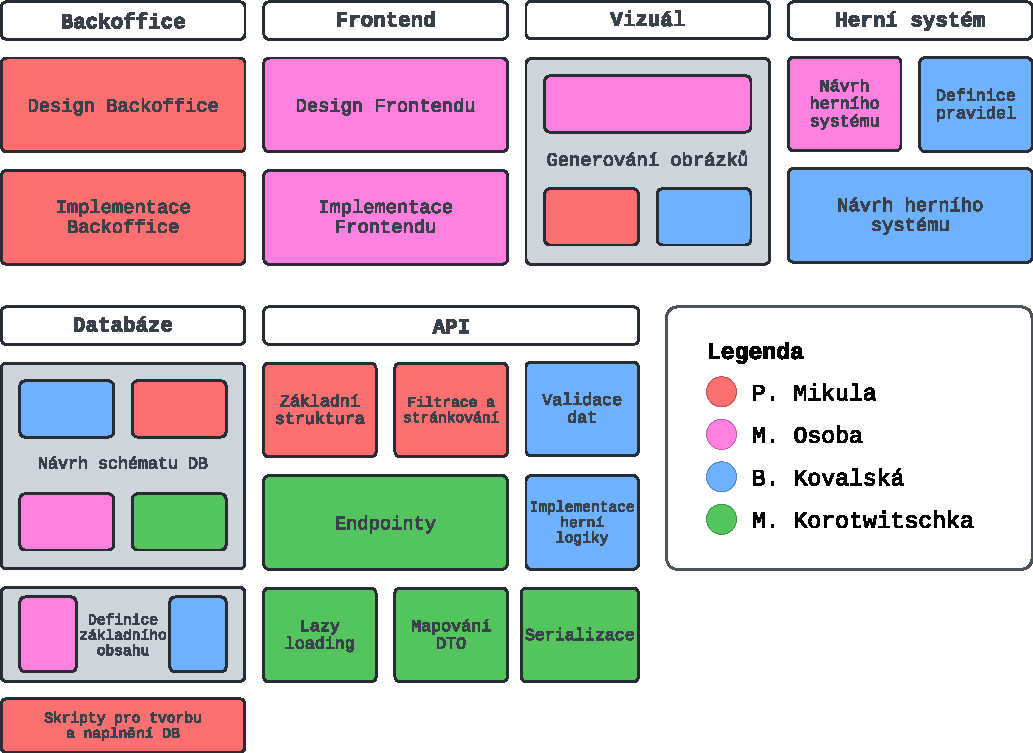
\includegraphics[width=\textwidth]{../../shared/diagrams/blocks.pdf}
    \caption{Rozložení práce v~týmu}
    \label{fig:job_distribution}
\end{figure}

Hlavními čtyřmi částmi projektu byla tvorba \textbf{administrativního rozhraní} (Pavel Mikula), \textbf{uživatelského prostředí} (Miroslav Osoba), \textbf{API} (Martin Korotwitschka) a~konečně implementace \textbf{herního modelu} (Barbora Kovalská), která je tématem této práce. Samotné vypracování však nebylo nutně omezeno pouze na tyto části, a~tak se v~průběhu vývoje mohlo stát, že se členové týmu podíleli i~na jiných částech projektu.

Rozvržení práce vyobrazeno na \customref{Obrázku}{fig:job_distribution} bylo provedeno především s~ohledem na zájmy a~schopnosti jednotlivých členů týmu, podle čehož se také v~prvé řadě přidělovalo samotné zadání bakalářské práce. V~samotném grafu byly tyto části rozděleny do bloků a~rozšířeny ještě o~dvě další sekce, které se ukázaly být dostatečně velké na to, aby se od ostatních osamostatnily -- \textbf{databáze} a~\textbf{vizuální vzhled} hry. 

Jednotlivé bloky znázorňují určitou část dané sekce, přičemž velikost daného bloku reprezentuje mohutnost tohoto úkolu. Dílčí části, na kterých se podílelo více členů týmu, jsou reprezentovány šedě s~barevnými bloky, jejichž velikost opět znázorňuje poměr práce jednotlivých spoluřešitelů.

Části projektu, na kterých se pracovalo v~této práci, budou popsány v~následujících kapitolách.

\subsection{Organizace projektu}
\label{subsec:versioning}

\begin{figure}[h]
    \centering
    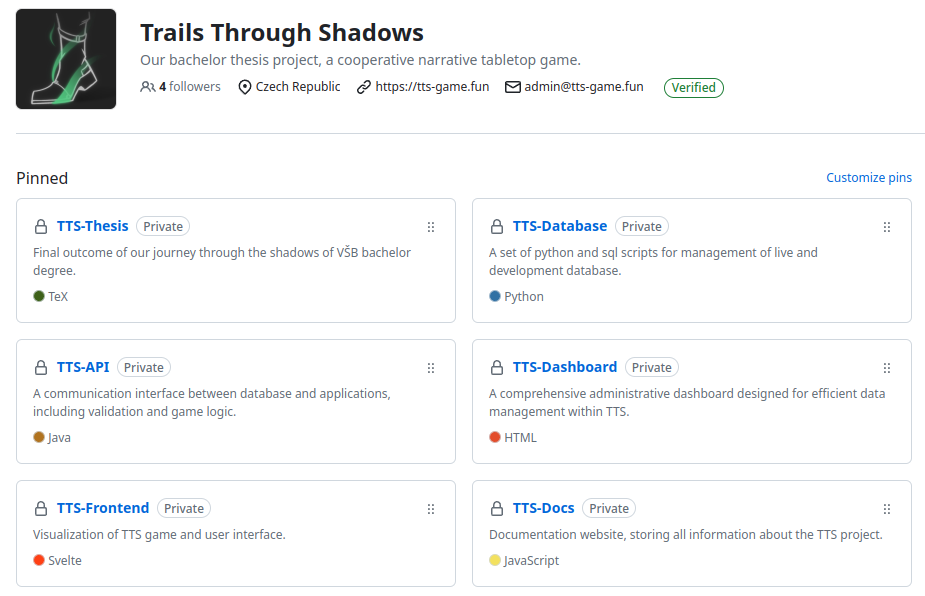
\includegraphics[width=\textwidth]{../../shared/figures/gitOrg.png}
    \caption{Rozdělení repozitářů v~rámci organizace}
    \label{fig:git_organization}
\end{figure}

Pro ucelení vývoje a~zajištění efektivní spolupráce byla v~rámci implementace vytvořena organizace \devTool{Trails Through Shadows}{https://github.com/Trails-Through-Shadows} na platformě \devTool{GitHub}{https://github.com}, kde byly vytvořeny repozitáře pro jednotlivé části projektu, jak je možné vidět na \customref{Obrázku}{fig:git_organization}. Organizace byla opatřena logem, které bylo vytvořeno v~rámci zadání práce a~bylo použito i~pro další potřeby týmu.

\begin{description}
    \item [TTS-Dashboard] -- Administrativní rozhraní sloužící ke správě hry, lokací, nepřátel a~dalších entit. Primární použití je pro vývojáře, kteří zde mohou vytvářet a~upravovat herní obsah.
    \item [TTS-Frontend] -- Uživatelské prostředí, které slouží k~interakci se hrou. Hráči zde mohou vidět své rozehrané kampaně a~postavy a~také vizualizaci celého souboje včetně herní mapy, iniciativního žebříčku a~nepřátel.
    \item [TTS-Api] -- \textit{API}, umožňující strukturovanou komunikaci mezi databází a~jednotlivými částmi hry. Obsahuje nejen základní \textit{CRUD} funkcionalitu, ale i~další metody pro komunikaci, autentizaci a~autorizaci, validaci vstupních dat a~také implementaci samotného herního systému pro správný chod hráčského prostředí.
    \item [TTS-Database] -- Nejedná se o~databázi jako takovou, neboť ta je hostována na serveru, ale o~skripty pro její vytvoření a~naplnění výchozích dat.
    \item [TTS-Docs] -- Dokumentace projektu, taktéž hostována na serveru, která schraňuje důležité informace, jež byly vytvářeny v~průběhu vývoje. Odkaz na ni je přiložen jako součást \texttt{README} souboru organizace a~je pomocí ní možné najít i~stránky ostatních části projektu.
    \item [TTS-Thesis] -- Repozitář pro bakalářskou práci, který obsahuje veškeré zdrojové kódy a~soubory potřebné pro vygenerování této práce. Každý z~členů týmu zde má svou vlastní složku, kde se nachází zdrojové kódy jeho dokumentu psané v~jazyce \LaTeX, a~také je zde složka \texttt{shared} obsahující společné soubory, jako jsou obrázky a~diagramy týkající se sdílených částí projektu.
\end{description}

Spolu s~organizací byla také zakoupena doména \texttt{tts-game.fun}, na kterou byly nasazeny veškeré části projektu, u~kterých to bylo přínosné. Kontinuální integrace byla prováděna při každém \textit{commitu} do hlavní větve repozitáře, kde byl vytvořen nový \textit{build} a~následně byl nasazen na server. Tento systém byl zajištěn pomocí služby \devTool{GitHub Actions}{https://github.com/features/actions} a~umožňoval všem členům týmu vidět aktuální stav projektu a~jeho vývoj.

Pro zvýšení přehlednosti a~efektivity souběžného vývoje tým využíval \devTool{Github Issues}{https://github.com/features/issues}, kde byly vytvářeny úkoly, které bylo možné přiřadit jednotlivým členům týmu. Co se týče větví, byl využit systém \texttt{master} -~\texttt{development} -~\texttt{feature}, pro úkoly tedy byla vytvořena tzv. \textit{feature branch}, kde byly prováděny změny, a~po dokončení byl vytvořen \textit{pull request} do \textit{development} větve, který byl po schválení sloučen i~do hlavní větve.

\section{Databáze}
\label{subsec:database}

Návrh databáze byl vysvětlen v~\customref{Kapitole}{sec:design_scheme}, kde byly popsány jednotlivé entity a~vztahy mezi nimi. Pro zjednodušení vývoje byl využit nástroj \devTool{dbdiagram}{https://dbdiagram.io/home}, který umožňuje vytvářet a~vizualizovat schémata databází a~následně je exportovat do souboru, který je možné použít pro skripty k~jejímu vytvoření. Pro implementaci byla zvolena databáze \devTool{MariaDB Server}{https://mariadb.org/}, která byla hostována na serveru a~byla přístupná primárně pomocí \textit{API}.

Na tvorbě návrhu se podíleli všichni členové týmu, kteří měli možnost navrhovat a~upravovat schéma databáze, a~také byli schopni vytvářet a~upravovat data v~databázi. Samotný návrh se v~průběhu vývoje měnil, a~to především kvůli změnám v~herním modelu, které byly zjištěny až při implementaci. O~případných změnách byli vždy všichni členové informováni včas a~u~těch s~většími zásahy se vedla diskuze, zda je změna nutná a~jaký bude její dopad na zbytek projektu. Pro testovací účely vznikla také vývojová databáze \texttt{tts\_api\_dev}, kde byly testovány nové změny před nasazením na produkci \texttt{tts\_api}.

V~rámci práce na projektu bylo také třeba definovat výchozí data, která dávala smysl jak z~herního hlediska, tak i~z~hlediska testování. Tento úkol byl svěřen těm členům týmu, kteří měli největší znalost herního modelu a~byli schopni vytvořit data, která byla pro testování dostačující. Pro začátek bylo tedy vytvořeno několik lokací, nepřátel a~čtyři rasy a~třídy, každá se svými jedinečnými akcemi a~efekty, které byly dostatečné pro testování základních funkcí hry. Data se do databáze vkládala pomocí skriptů napsaných v~jazyce \devTool{Python}{https://www.python.org/}, které jako vstup přijímaly soubory ve formátu \texttt{JSON} a~následně je vkládaly do databáze.

\section{Vizuál hry}
\label{subsec:game_visuals}

Na vizuální stránce hry se podílel především člen týmu zodpovědný za uživatelské rozhraní, jisté úkoly, především tvorba obrázků, zde však byly delegovány i~na jiné členy týmu. Pro vytvoření vizuálně atraktivní hry bylo třeba vytvořit obrázky pro lokace, předměty, nepřátele, rasy a~třídy, a~také pro každou kombinaci, která může vzniknout při tvorbě postavy. V~rámci vývoje bylo rozhodnuto o~použití generátoru \devTool{Midjourney}{https://www.midjourney.com/home}, který umožnil rychlé a~jednoduché vytvoření obrázků, které byly následně použity v~herním prostředí.

Jako největší problém se ukázalo udržení vizuální konzistence, což zčásti vyřešilo zavedení pevné struktury dotazů na obrázky. I~tak však nebylo úplné konzistence dosaženo. Pro budoucí vývoj by bylo vhodné zajistit jednotnou grafiku a~zvážit možnost vytvoření vlastních obrázků.

Pro zvýšení přehlednosti byly obrázky rozděleny do složek podle jejich typu a~názvu a~v~\textit{API} byly vytvořeny metody, které umožňují získat obrázek podle jeho názvu, což zjednodušilo práci s~obrázky v~herním modelu.

\subsection{Efekty}
\label{subsec:effects}

Efekty \imageref{fig:effects} byly vytvořeny pomocí výše zmíněného generátoru \textit{Midjourney}, pokud bylo třeba, byly upraveny v~programu \devTool{GIMP}{https://www.gimp.org/}, následně převedeny do formátu \texttt{SVG} a~vyladěny pomocí programu \devTool{Inkscape}{https://inkscape.org/}. Důraz byl kladen především na jedinečnost a~rozličnost siluet, neboť tyto ikony byly dále použity na kartách v~malých rozměrech.

Je důležité zmínit, že ve finální hře se nepoužily všechny efekty, které byly popsány v~návrhu \chapterref{subsec:design_effects}. Během testovacích herních sezení se totiž zjistilo, že jejich počet je pro hru příliš velký a~zbytečně ji zdržuje. Byly tedy vybrány ty nejzákladnější a~nejčastěji se vyskytující efekty.

\begin{figure}[H]
    \centering
    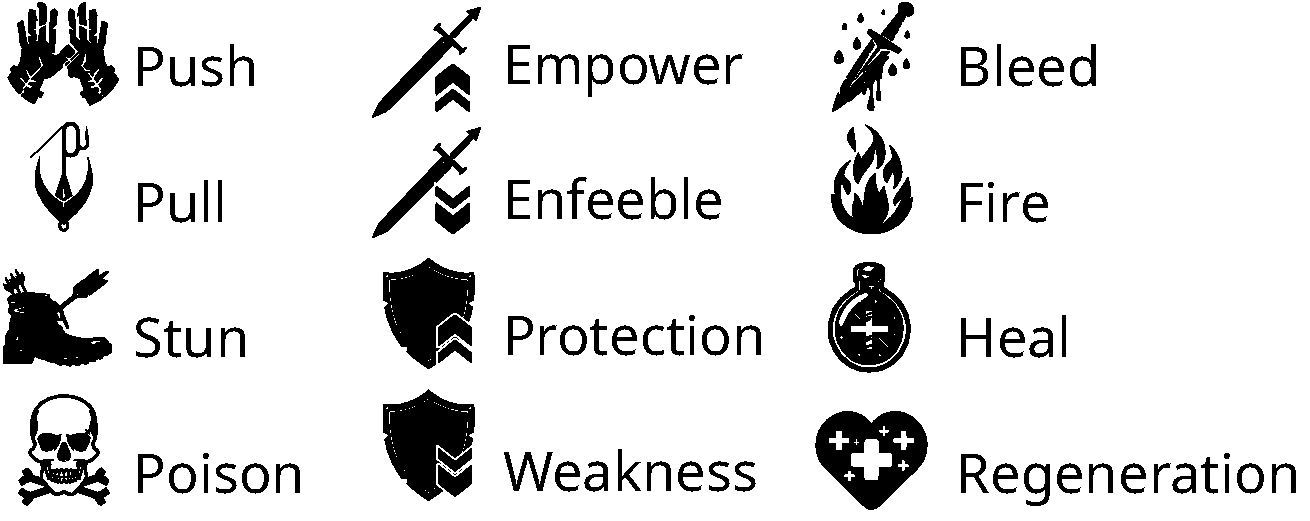
\includegraphics[scale=0.7]{figures/images/effects.pdf}
    \caption{Ikony efektů}
    \label{fig:effects}
\end{figure}

Rezistence byly vytvořeny pouhým přeškrtnutím korespondujícího efektu. Pro efekty \textit{Push} a~\textit{Pull} byla pro zjednodušení vytvořena jedna rezistence s~názvem \textit{Forced Movement Resistance}, která byla následně použita pro oba efekty. Na \customref{Obrázku}{fig:resistances} je jako příklad zobrazena právě tato rezistence spolu s~rezistencí na efekt \textit{Stun}.

\begin{figure}[H]
    \centering
    
\includegraphics[scale=0.7]{figures/images/resistances.pdf}
    \caption{Ikony rezistencí}
    \label{fig:resistances}
\end{figure}

\subsection{Karty}
\label{subsec:cards}

Pro zjednodušení práce při tvorbě nových akcí bylo důležité implementovat dynamickou tvorbu uživatelsky příjemných a~přehledných karet, které by pak byly v~případě akcí nepřátel určeny k~zobrazování v~uživatelském rozhraní a~pro hráčské akce byly vytisknuty a~použity fyzicky. Výsledek je možné vidět na \customref{Obrázku}{fig:cards}.

\begin{figure}[H]
    \centering
    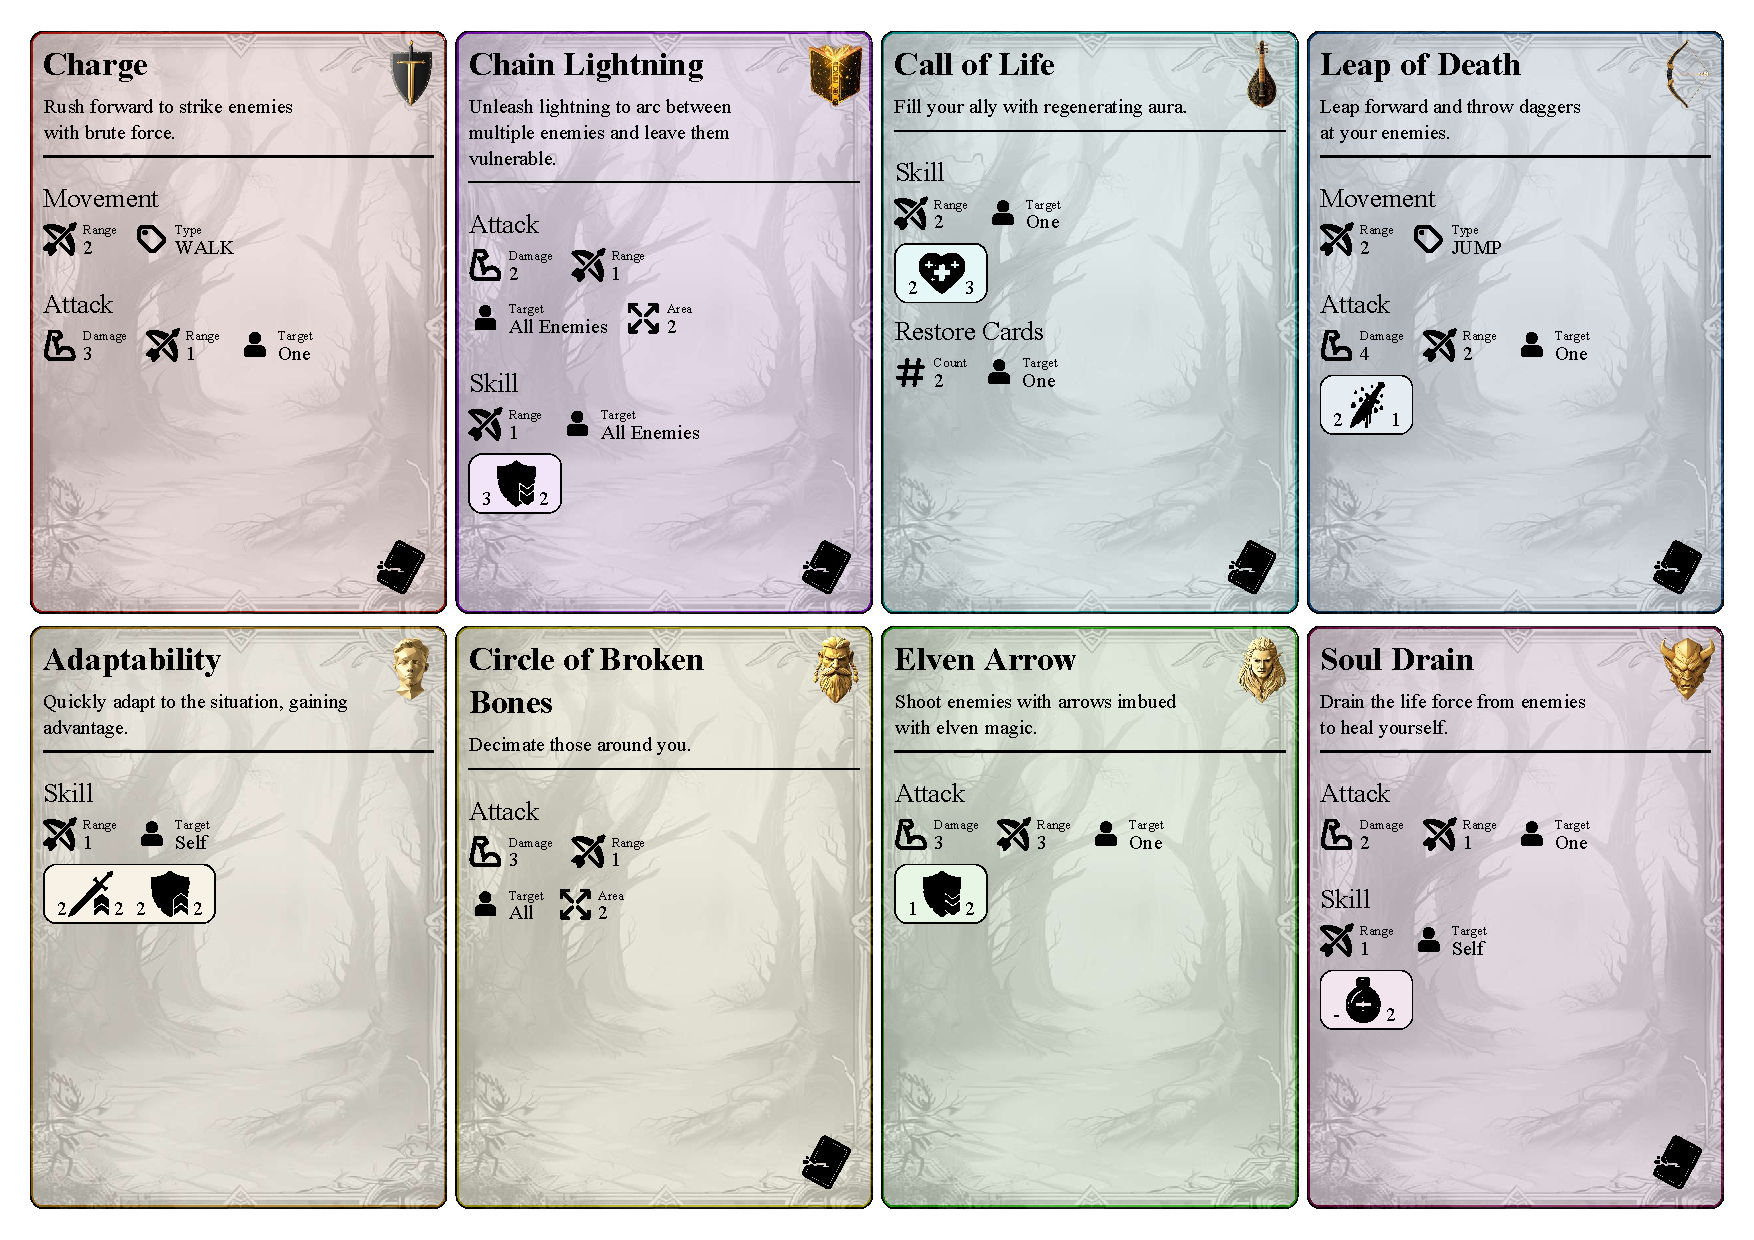
\includegraphics[width=\textwidth]{figures/images/cards.pdf}
    \caption{Karty akcí}
    \label{fig:cards}
\end{figure}
\newpage

Dynamické vykreslování karet bylo napsáno v~jazyce \devTool{JavaScript}{https://www.w3schools.com/js/} zajištěno pomocí knihovny \devTool{SVG.js}{https://svgjs.dev/docs/3.0/}, která umožňuje vytvářet a~manipulovat s~vektorovými obrázky, kde byl výsledek ve formátu \texttt{SVG} skvělou volbou pro tisk a~zároveň bylo možné ho použít i~pro zobrazení v~uživatelském rozhraní. Jednodušší ikony byly získány z~open-source knihovny \devTool{SVGrepo}{https://www.svgrepo.com/}, pro obrázky zdroje karty (rasa nebo třída) a~pro efekty byly použity dříve vytvořené ikony.

Vytvořená funkcionalita tak dokázala dynamicky generovat karty pro jednotlivé akce, které byly následně použity v~administrativním rozhraní, uživatelském prostředí i~pro tisk.

\subsection{Fyzické Komponenty}
\label{subsec:physical_components}

Fyzické komponenty byly nejprve vymodelovány v~programu \devTool{Blender}{https://www.blender.org/}, kde byly v~rámci této práce vytvořeny modely pro části lokace, stojany pro postavy a~nepřátele a~žetony překážek a~dveří. Jednotlivá políčka herní desky a~stojanů obsahovaly otvory pro magnety, které zajišťovaly příjemné připevnění figurek na hexagony. Na \customref{Obrázku}{fig:game_board} je přiložen \textit{render} herní desky, která byla vytvořena z~těchto modelů.

\begin{figure}[h]
    \centering
    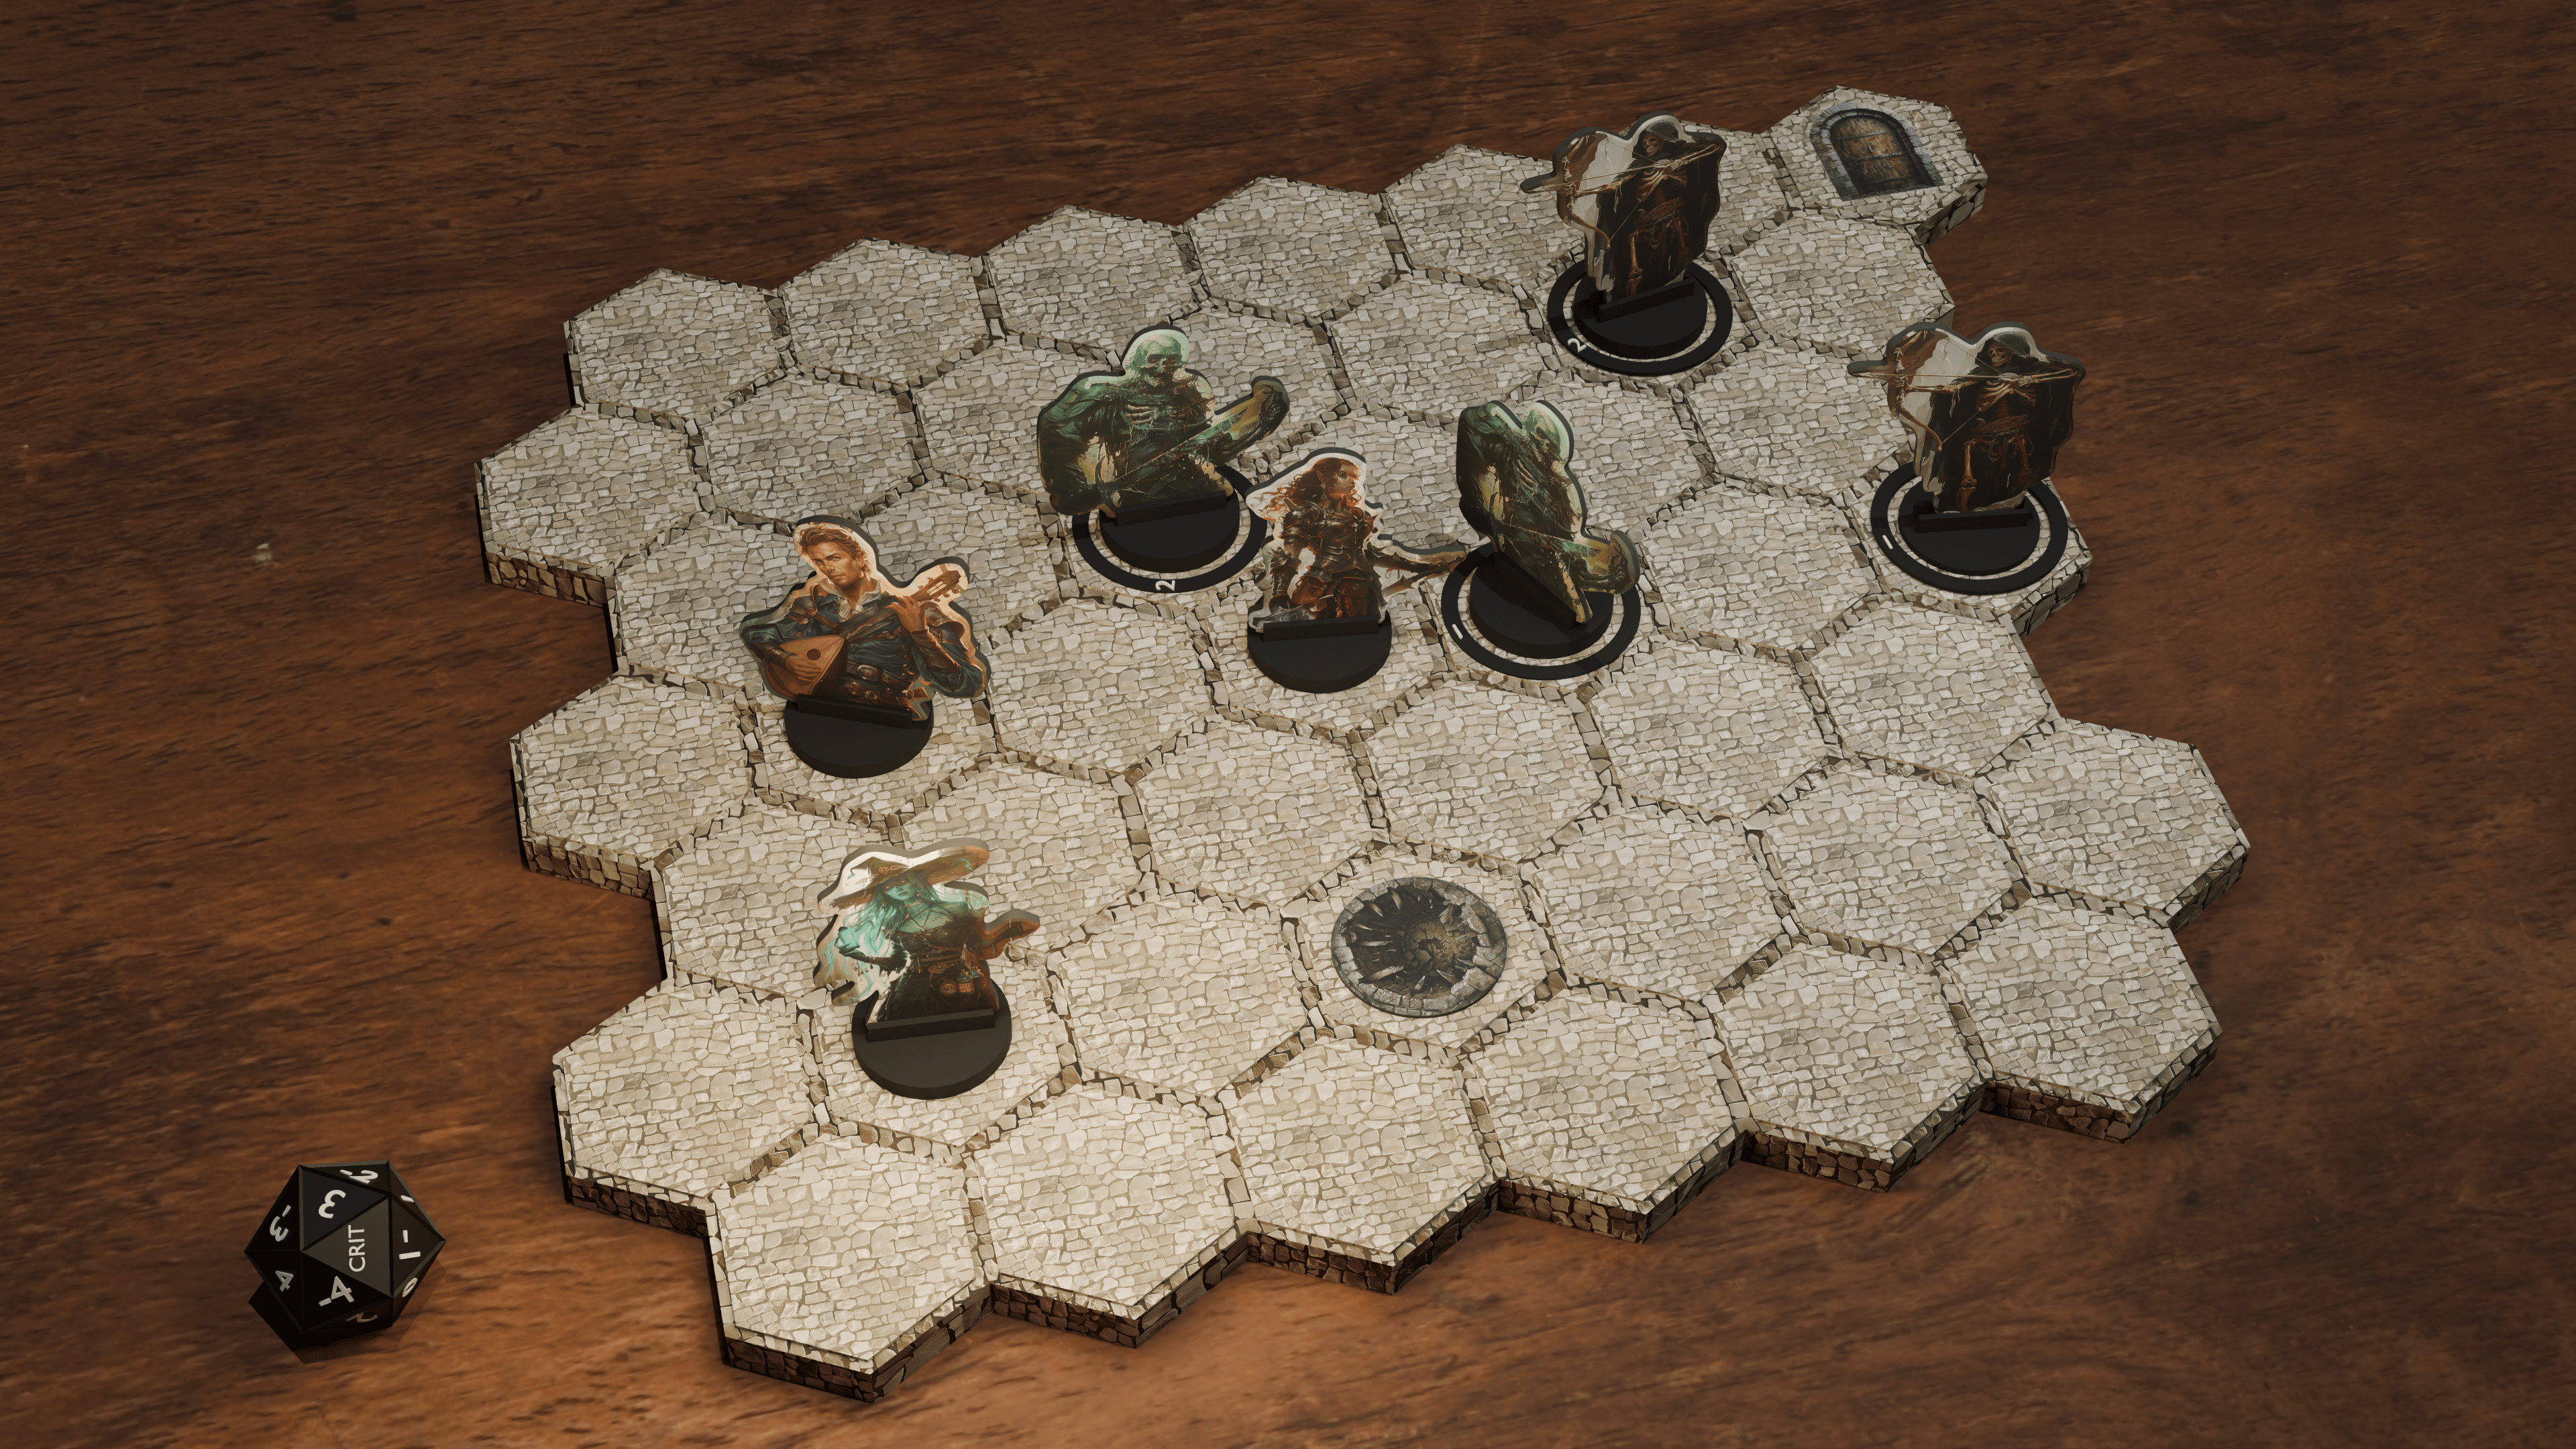
\includegraphics[width=\textwidth]{figures/images/game.png}
    \caption{Herní deska s~fyzickými komponenty}
    \label{fig:game_board}
\end{figure}

Tyto modely byly následně předány jiným členům týmu, kteří se postarali o~jejich správné vytištění a~následnou instalaci magnetů. Na herní pole a~žetony byly nalepeny samolepky s~obrázky, postavy a~nepřátelé byli vytisknuti na pevný papír dost široký na to, aby je bylo možné vložit do stojanu.

\section{Implementace herní logiky}
\label{sec:game_logic}

Hlavním bodem, který tato práce řeší, je implementace herního modelu, který je základem celé hry. Tato část byla provedena v~rámci \textit{API} projektu, jak již bylo zmíněno výše, a~byla napsána v~jazyce \devTool{Java}{https://www.java.com/}. Pro přehlednost byla herní logika oddělena od ostatních zdrojových kódů \textit{API} do samostatné složky \texttt{algorithm}, kde byly vytvořeny třídy pro jednotlivé entity a~metody pro jejich manipulaci.

V~rámci projektu \textit{API} bylo využito mnoho knihoven, které umožnily snadnou práci s~daty a~zároveň zajišťovaly bezpečnost a~efektivitu. Pro implementaci herní logiky byly použita především knihovna \devTool{Lombok}{https://projectlombok.org/}, která umožňuje snadnou tvorbu metod \texttt{getter}, \texttt{setter} a~\texttt{constructor}, dále pomocná knihovna \devTool{Jackson}{https://www.baeldung.com/jackson} pro práci s~\texttt{JSON} daty a~knihovna \devTool{Swagger}{https://swagger.io/}, zajišťující dokumentaci koncových bodů \textit{API}.

Další problém stojící za zmínku je časová náročnost implementace veškerých herních modelů. Vzhledem k~tomu, že se jedná o~relativně komplexní systém, bylo třeba věnovat dostatečný čas na implementaci a~testování, což se ukázalo být časově nákladnější, než bylo původně plánováno. Z~tohoto důvodu bylo rozhodnuto o~zjednodušení některých částí herního modelu, což zahrnovalo snížení počtu efektů a~odložení implementace poskoků a~předmětů na potenciální rozšíření hry v~budoucím vývoji. Vývojový tým se však shodl na potenciálu, který tato hra má, proto bylo rozhodnuto o~pokračování v~jejím vývoji i~mimo rámec této práce.

Nejdůležitější funkcionality této části projektu jsou rozebrány v~následujících kapitolách.

\subsection{Session}
\label{subsec:impl_session}

První částí, která byla implementována, byla třída \texttt{Session} spolu s~nadřazenou správní třídou \texttt{SessionHandler}, která zajišťuje správu přihlašovacích relací a~byla navržena tak, aby bylo možné vytvářet nové relace, ukládat do nich data a~následně s~nimi pracovat. Třída obsahuje metody pro vytvoření nové relace, získání relace podle identifikátoru, a~případné odhlášení. Samotná třída \texttt{Session} obsahuje informace o~uživateli, který je přihlášen, a~také klíč relace, který se používá k~její identifikaci. Tato třída se dále využívá pro kontrolu, zda má uživatel přístup na dobrodružství, se kterými se snaží pracovat.


\subsection{Entity}
\label{subsec:impl_entity}

Pro jednoduchou reprezentaci entit (postavy, nepřátelé, překážky a~poskoci) byla vytvořena třída \texttt{Entity}, která tyto modely zaobaluje a~umožňuje s~nimi snadno pracovat. Třída obsahuje sadu dvou identifikátorů -- jeden pro identifikaci samotného objektu a~druhý pro číslo skupiny, což se používá u~nepřátel, se kterými je třeba pracovat v~obou možnostech. Dále obsahuje informace o~životě, obraně, iniciativě a~také seznam efektů, které na entitu působí.

Mezi metodami třídy \texttt{Entity} jsou ty zajišťující práci s~efekty, zranění a~léčení a~vyhodnocení začátku a~konce tahu. Třída je zobrazena ve \customref{Výpisu}{code:entity}.

\begin{listing}[H]
    \inputminted{Java}{code/EncounterEntity.java}
    \caption{Zdrojový kód třídy Entity}
    \label{code:entity}
\end{listing}


\subsection{Encounter}
\label{subsec:impl_encounter}

Pro samotnou správu souboje byla vytvořena třída \texttt{Encounter}, která obsahuje informace o~jednotlivých hráčích, nepřátelích, iniciativním žebříčku, detailech lokace, na které souboj probíhá, požadavky pro ukončení daného souboje a~mnoho dalších vlastností, popisujících momentální stav souboje. Při každém volání požadavku na jakoukoli interakci se soubojem se kontroluje, zda klíč relace předaný v~hlavičce odpovídá licenčnímu klíči, což zajišťuje, aby hráči nebyli schopni manipulovat s~daty, ke kterým nemají přístup. 

Průběh souboje funguje podle postupu popsaného v~\customref{Kapitole}{subsec:design_encounter}, jeho funkcionalita byla implementována v~rámci \textit{API} a~lze s~ním interagovat pomocí koncových bodů (dále jen \textit{endpoint}) třídy \texttt{EncounterController}, které jsou zobrazeny v~\customref{Tabulce}{tab:endpoints}, kde byly pro přehlednost vybrány pouze ty nejdůležitější. Jsou logicky rozděleny do pěti skupin, kde každá skupina obsahuje \textit{endpointy} pro práci s~určitou částí souboje. Tato část projektu tedy zajišťuje jednoduché a~efektivní řešení pro práci s~herním modelem, kde je kontrolováno jak správné pořadí operací, tak i~správnost vstupních dat.

\begin{table}[h]
    \centering
    \resizebox{\textwidth}{!}{%
    \begin{tabular}{>{\bfseries}r >{\ttfamily}l >{\ttfamily}l >{\ttfamily}H l}
        \toprule
        
        Metoda & 
        \normalfont{\textbf{Endpoint}}
            \tablefootnote{Cesty ke všem endpointům začínají na adrese \texttt{/encounter}.} & 
        \normalfont{\textbf{Vstup}}
            \tablefootnote{Kromě \texttt{idLocation}, který je předán jako parametr URL, je vstup přijímán ve formátu JSON jako tělo požadavku.} & 
        \normalfont{\textbf{Výstup}} & 
        \textbf{Popis} \\
        \midrule
        
        POST & /\{idAdventure\} & idLocation & idEncounter & Vytvoření encounteru \\
        GET & /\{id\} & & Encounter &  Získání daného encounteru \\
        GET & / & & List<Encounter> & Získání všech encounterů \\
        DELETE & /\{id\} & & & Odstranění daného encounteru \\
        GET & /\{id\}/status & & EncounterState & Získání statusu encounteru \\
        \midrule

        POST & /\{id\}/initiative & List<Initiative> & & Počáteční hod na iniciativu \\
        GET & /\{id\}/initiative & & List<Initiative>, ActiveEntity & Získání iniciativy \\
        \midrule

        POST & /\{id\}/openDoor & Door & & Otevření dveří \\
        POST & /\{id\}/endRound & & UnlockedParts, EncounterState & Ukončení kola \\
        \midrule

        POST & 
            /\{id\}/turn/character/\{idCharacter\}/start 
            & & EntityStatusUpdate & Začátek tahu hráče \\
        POST & 
            /\{id\}/turn/character/\{idCharacter\}/end 
            & & EntityStatusUpdate & Konec tahu hráče \\
        POST & 
            /\{id\}/turn/enemy/\{idEnemy\}/start 
            & & List<EntityStatusUpdate>, Action & Začátek tahu nepřítele \\
        POST & 
            /\{id\}/turn/enemy/\{idEnemy\}/end 
            & & List<EntityStatusUpdate> & Konec tahu nepřítele \\
        \midrule

        POST & 
            /\{id\}/interaction/character/\{idCharacter\} & 
            Interaction & EntityStatusUpdate & Interakce s hráčem \\
        POST & 
            /\{id\}/interaction/enemy/\{idGroup\}/\{idEnemy\} & 
            Interaction & EntityStatusUpdate & Interakce s nepřítelem \\
        
        \bottomrule
    \end{tabular}}
    \caption{Seznam endpointů pro práci s encounterem}
    \label{tab:endpoints}
\end{table}

První skupina obsahuje metody pro práci se samotným soubojem. Vytvoření efektu přijímá jako parametry \texttt{id} dobrodružství a~lokace, na kterou hráči zamířili. V~systému dojde k~nastavení všech proměnných souboje, včetně ukončovacích podmínek a~seznamu hráčů, také je zde odhalena první startovací část mapy, která je zobrazena hráčům. Další \textit{endpointy} slouží k~získání informací o~souboji, jeho stavu a~také k~jeho ukončení.

Po vytvoření je třeba nejprve určit iniciativní pořadí, což je zajištěno pomocí \textit{endpointů} druhé skupiny, které přijímají seznam iniciativ hráčů a~následně je zpracovávají. Pro nepřátele si systém iniciativu vypočítá sám a~následně je možné získat pořadí pomocí \textit{endpointu}, který vrací seznam iniciativních hodnot a~momentálně aktivní entitu.

Další skupina se stará o~práci s~kolem. Otevření dveří je zajištěno pomocí \textit{endpointu}, který zpracuje požadavek na otevření dveří a~uloží je do seznamu. Během konce kola jsou pak všechny zaznamenané dveře otevřeny a~je zjištěn nový stav mapy, který je spolu s~novým stavem souboje zobrazen hráčům.

Čtvrtá skupina se stará o~práci s~tahy entit. U~začátku a~konce tahu hráče systém přijímá pouze jeho \texttt{id} a~podle něj pak u~dané postavy provede potřebné změny. Nepřátelé začínají kolo jako skupina, proto systém provede změny pro každého nepřítele v~dané skupině. V~obou možnostech \textit{endpointy} vrací objekt nebo seznam objektů \texttt{EntityStatusUpdate}, který obsahuje informace o~změnách, kterými entita prošla, ovšem u~nepřátel je přidána ještě akce, kterou nepřátelé ve svém tahu zahrají.

Poslední skupina týkající se interakce s~entitami je opět rozdělena na hráče a~nepřátele. Spolu se vstupem je zde přijímán objekt \texttt{Interaction}, který obsahuje informace o~zranění, které entita dostala, a~seznam efektů, které je na ni třeba aplikovat. Pro hráče stačí předat pouze jedno \texttt{id}, u~nepřátel je situace složitější, protože jsou identifikováni jak podle skupiny, ke které patří, tak jejich pořadím v~dané skupině. Je tedy potřeba předat \texttt{id} skupiny a~\texttt{id} nepřítele, což systém zpracuje pro odpovídající entitu. Výstupem je opět objekt \texttt{EntityStatusUpdate}.

\section{Validace dat}
\label{sec:validation}

Druhou nezanedbatelnou částí, která byla v~\textit{API} implementována, je validace dat. Pro zajištění konzistence a~bezpečnosti bylo nutné zkontrolovat, zda data, která jsou vkládána do databáze, splňují požadavky, které byly stanoveny v~návrhu.

Seznam validací, které se provádí pro jednotlivé modely, byl kromě samotného zdrojového kódu souběžně veden ve výše zmíněné dokumentaci, aby byl tento proces transparentní. Pro ukázku je zde přiložen seznam validačních požadavků pro část lokace (interně nazvaný \texttt{Part}).

\begin{itemize}
    \setlength\itemsep{0.5mm}
    \item Název a~štítek musí být platné.
    \item Část musí mít nejméně 5 a~nejvíce 50 hexagonů.
    \item Každý hexagon musí být ověřen.
    \item Část musí mít šířku maximálně 8 hexagonů ve všech směrech.
    \item Žádné hexagony se nesmí překrývat.
    \item Část musí obsahovat středový hexagon (0, 0, 0).
    \item Všechny hexagony musí být propojeny.
\end{itemize}

\begin{listing}[h]
    \inputminted{Java}{code/Validable.java}
    \caption{Zdrojový kód třídy Validable}
    \label{code:validable}
\end{listing}

Na \customref{Výpisu}{code:validable} je zobrazena třída \texttt{Validable}, která je základem pro všechny modely, které potřebují validovat svá data. Třída obsahuje metodu \texttt{validate}, která je volána při vkládání nového záznamu do databáze a~zajišťuje spuštění interní kontroly daného objektu. Tato metoda interně volá \textit{protected} metodu \texttt{validateInner}, která je implementována v~každé třídě zvlášť a~zaručuje, že data splňují požadavky, které jsou specifické pro daný model. Zbytek této metody jen zajišťuje zaobalení a~v~případě zachycení chyby tyto informace předává dále.

Validace dále pokračuje v~samotné třídě \texttt{Part}, která je zobrazena na \customref{Výpisu}{code:part}, do kterého byly vybrány jen některé z~kontrol, opravdová třída však obsahuje všechny kontroly zapsané ve výše uvedeném seznamu. Třída obsahuje metodu \texttt{validateInner}, která zajišťuje, že data splňují požadavky, které byly pro části lokací stanoveny. V~této metodě je zkontrolováno, že má část validní název i~štítek, minimální počet hexagonů, že obsahuje středový hexagon a~že jsou všechny hexagony propojeny. V~případě, že některá z~těchto podmínek není splněna, je vyhozena výjimka \texttt{ValidationError}, která obsahuje informace o~chybě jako obecnou chybovou hlášku, jméno objektu, jméno nevalidního pole a~odmítnutou hodnotu.

Za zmínku také stojí parametr třídy  \texttt{ValidationConfig}, který se předává při volání této metody a~obsahuje různé informace, vůči kterým se objekt validuje. Na výpisu se tato konfigurace používá pro předání minimálního počtu hexagonů a~také se posílá do metody \texttt{validateChild}, která zajišťuje kontrolu vnitřních objektů, jako je název a~štítek.

\begin{listing}[H]
    \inputminted{Java}{code/Part.java}
    \caption{Zdrojový kód třídy Part}
    \label{code:part}
\end{listing}

\newpage
\section{Herní příručka}
\label{sec:game_manual}

Na závěr celého vývoje byla vytvořena herní příručka přiložená v~\customref{Příloze}{chap:rulebook}, která obsahuje veškeré informace o~hře, které hráči potřebují k~jejímu odehrání vědět. Byla vytvořena pomocí nástroje \devTool{Homebrewery}{https://homebrewery.naturalcrit.com/}, který umožňuje vytvářet dokumenty v~stylu \dnd{}. Aby se příručka od tohoto velmi známého formátu odlišovala, byly použity vlastní obrázky a~styly, které byly vytvořeny v~rámci projektu. Podobně jako ostatní herní materiály byla i~tato příručka napsána v~anglickém jazyce.

Dokument začíná krátkým úvodem, který nastiňuje atmosféru herního světa, do kterého se hráči plánují ponořit. Okamžitě je také zmíněna klíčová role podpůrné aplikace spolu s~odkazem, na kterém ji hráči mohou nalézt. Na druhé straně je přiložen obrázek herních komponent spolu s~vysvětlivkami jednotlivých částí a~také je zde popsána struktura karty. Je zde také stručný postup pro přípravu herní kampaně a~souboje, kde jsou hráči odkázáni především na podpůrnou aplikaci, která je tímto procesem provede.

Následně se příručka věnuje samotné hře, představí hráčům systém akcí a~popíše, jakým způsobem mají provádět jednotlivé prvky. Následně jsou spolu s~přehledným obrázkem představeny všechny efekty, které se ve hře mohou vyskytnout, a~v~tabulce jsou uvedeny jejich názvy, popisy a~také to, zda na ně hráči mohou získat rezistenci. Výběr ras a~tříd zde přiložen není, neboť jejich popis je dostupný v~podpůrné aplikaci, která je hráčům k~dispozici. Po představení herních mechanismů jsou popsány instrukce ke správnému odehrání hráčského a~nepřátelského kola. Sekce zaměřená na hru končí popisem ukončení souboje, spolu s~výčtem možných ukončovacích podmínek a~výsledky, které z~nich vyplývají.

Příručka končí krátkým povzbuzujícím závěrem, který má hráče motivoval k~dalšímu hraní, a~také obsahuje poslední přání od vývojového týmu, který se na projektu podílel. Celý dokument je napsán v~jednoduchém a~srozumitelném stylu, který hráčům usnadňuje orientaci a~současně je zaujme. Příručka bude hráčům k~dispozici v~elektronické podobě na stránce dokumentace projektu popsané v~\customref{Kapitole}{subsec:versioning} a~bude také vytisknuta a~přiložena k~fyzickým komponentům hry.


% not representable enough
% \lstinputlisting[%
%     language=Java,%
%     label=src:validationError,%
%     caption={Zdrojový kód třídy ValidationError}]%
%     {code/ValidationError.java}
